Da der Schwerpunkt dieser Arbeit auf dem Umgang mit Konflikten der zu testenden Technologien liegt, soll die Bedienoberfläche der Anwendung möglichst einfach gehalten werden.\\
Alle Adressbucheinträge sollen in einer Liste angezeigt werden. Zum Anlegen, Editieren und Löschen eines einzelnen Eintrags soll es eine zweite Ansicht geben, auf die man per Klick auf den entsprechenden Eintrag in der Liste gelangt.
Wenn es zum Konflikt kommt, kann dieser über ein Dialogfenster von den NutzerInnen aufgelöst werden.
Im Dialog muss erkennbar sein bei welchem Kontakteintrag der Konflikt auftrat.
Außerdem müssen sich die entsprechenden Bereiche beider Versionen unterscheiden lassen und auswählbar sein. \autoref{fig:dialog} zeigt, wie so ein Dialogfenster aussehen könnte.
%
\begin{figure}[H]
	\centering
	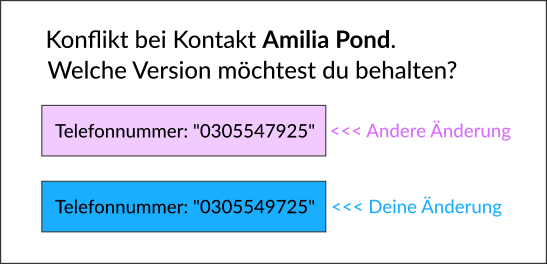
\includegraphics[width=0.8\textwidth]{Konfliktdialog}
	\grayRule
	\caption{Dialogfenster im Konfliktfall}
	\label{fig:dialog}
\end{figure}
%
Wurde beispielsweise Amilias Telefonnummer von zwei Personen gleichzeitig bearbeitet, bildet der Dialog zwei Bereiche mit der Nummer in den unterschiedlichen Versionen ab.
Daneben ist abzulesen woher die Änderung stammt.
Die lokal gespeicherte Version kann mit ''Deine Änderung'' betitelt werden, die Version, die vom Server kommt mit ''Andere Änderung''.
Durch einen Klick auf den Knopf mit der Telefonummer kann entschieden werden welche als korrekte Version behalten wird.